\documentclass{standalone}
% preamble: usepackage, etc.
\begin{document}

\chapter{强化学习基础}

强化学习是一种学习如何进行控制和决策的框架,强化学习的灵感来自于仿生学,它完成了从当前的环境状况到行为的映射,并通过学习这一映射过程使得从环境中得到的奖赏值最大化。这样一种框架被誉为可能是发展为强人工智能的框架,包括博弈论、控制理论、群体智能、多智能体系统等领域都与强化学习可以进行结合和交叉。在控制领域,强化学习被视为一种拟合动态规划方法。在博弈论领域,它被用来解释均衡点的出现及其原因。它和有监督学习,无监督学习组成了机器学习领域三个基本的学习框架。强化学习不同于有监督学习和无监督学习,原因在于在强化学习中,并不存在类似于有监督学习中的标签信息,只有奖赏信号用于指导整个学习过程,同样这也不同于无监督学习中没有任何信号和标签指导学习过程。\par

\section{智能体建模方法和马尔科夫决策过程}
\subsection{智能体建模方法}
强化学习框架的设计一般基于智能体建模的方式实现,基于智能体的模型是一种为了模拟控制和交互的计算模型,这样一种框架包括智能体和环境两类主体,其在多个领域都有广泛的应用,如在生物学中用于研究种群的分布,人口变化等问题,在经济和社会学中,用于研究城市人口流动和城市规划问题,消费者行为分析等。在强化学习中,我们通过图4-1所示的框架\citing{R2005Reinforcement}对强化学习进行建模。Agent 表示智能体,即表示我们的控制算法的主体。Environment 表示环境,智能体与环境进行交互。在路径规划问题中,智能体代表了我们的路径规划算法,它输出控制车辆的行为如直行,左转等,而环境代表了实际的地图环境,如我们在第2章节所述的多个场景等。
\begin{figure}[H]
	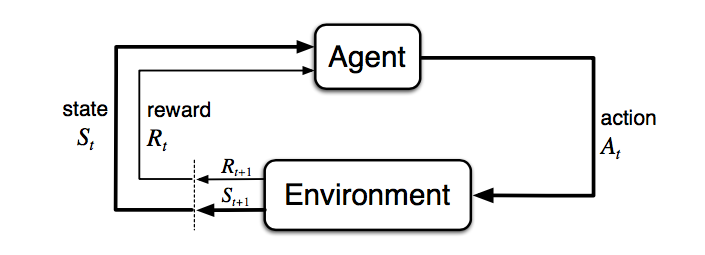
\includegraphics[width=12.0cm]{pic/4-1.png}
	\caption{强化学习框架}
	\label{4-1}
\end{figure}
\subsection{马尔科夫决策过程}
马尔科夫决策过程(Markov Decision Process, MDP)为建模决策问题提供了一个数学框架,马尔科夫决策过程对于通过动态规划或强化学习解决和研究优化问题十分重要。这一框架最早于1950年提出,随后 Ronald A. Howard 在书中做了详细做了详细的研究\citing{FosterDynamic}。
在强化学习中,我们通常把环境规范到马尔科夫决策过程,这样的设计有利于强化学习算法的设计,同时便于算法的相关理论证明。\par
精确的来说,智能体和环境在一个离散的时间序列$t=0,1,2,3,... ..$上进行交互,在一个时刻$t$上,智能体接受到表示环境状态的信息(State),随后根据自己身的策略和决策系统,给出行为(Action)。环境在接收到该行为后,依据某一概率转移矩阵(P),进行状态的更新,同时计算一个对应的奖赏信号(Reward),环境把新的状态和奖赏信号返回给智能体,此时进入下一个时刻,该过程不断重复直到环境返回一个结束信号(Terminal Signal)。因此根据以上描述,我们定义一个马尔科夫决策过程是一个包含5个元素的元组,表示为$MDP=(S, A, P, R, \gamma)$,其中$S$为一个表示状态的有限集合。$A$表示一个行为的有限集合,更特别的用$A_s$表示某一状态$s$下的可取的行为的集合。$P(s, s',a) = \mathbb{P}(s_{t+1} = s'|s_t = s, a_t=a)$表示在$t$时刻,状态为$s$,采用行为$a$时,$s_{t+1}$为$s'$的概率。$R(s, s', a)$表示在$t$时刻,状态为$s$,采用行为$a$,状态转移到$s'$时,环境的即时奖赏值。$\gamma \in [0, 1]$表示折扣因子,表示我们主观对即时奖赏和未来奖赏重要程度的差别。\par 

\section{强化学习}
强化学习的目标在于找到一个策略(Policy),使得在该策略下,智能体能够最大化其从环境中受到的累计奖赏值(Long-Term Reward)。因此在控制或者决策问题中,我们假设我们的目标或目的即为最大化累计奖赏,这一假设称为奖赏假设。而这一形式也是强化学习相比于其他机器学习框架独特所在。\par
策略定义为:$\pi(a|s) = \mathbb{P}[a_t=a | s_t=s]$,即策略为一个给定状态的行为的概率分布。策略完全定义了一个智能体的行为,同时其决策只依赖于当前时刻的状态。
因此在一个决策过程中,给定$MDP=(S, A, P, R, \gamma)$ 和$\pi(a|s)$,智能体和环境进行交互,最终产生一条轨迹(Trajectory),定义为: $s_0, a_0, r_0, s_1, a_1, r_1, ...$。对于这样一个元组$(s_t, a_t, s_{t+1}, r_{t+1})$我们定义其为一个样本(sample)或者转变(transition)。它强化学习中进行学习的一个最小样本。同样,如果我们得到的某条轨迹是采样直到收到了环境的终止信号,则成该轨迹为一个完整的节(Episode)。如前面所述,智能体的目标在于最大化累计奖赏,累计奖赏的定义如下:
\begin{center}
    \begin{equation}
        G_t=r_{t+1} + \gamma r_{t+2}+... = \sum_{k=0}^{\infty}\gamma^{k}R_{t+k+1}
    \end{equation}
\end{center}
\subsection{价值函数}
在这一节,我们将介绍强化学习中一个重要的函数,价值函数,它表示了对一个状态的好坏程度的估计值,好坏被严格定义为在该状态下累计奖赏期望的大小。\par
状态价值函数$v_{\pi}(s)$表示以状态$s$作为初始状态,按照策略$\pi$进行决策下,智能体所受到的累计奖赏值。即:
\begin{center}
    \begin{equation}
        v_{\pi}(s) = \mathbb{E}_{\pi}[G_t|s_t=s] = \mathbb{E}[\sum_{k=0}^{\infty}{\gamma^k{R_{t+k+1}}}|s_t=s]
        \mbox{, for all s $\in$ S.}
    \end{equation}
    \mbox{其中$\mathbb{E[\cdot]}$表示给定策略$\pi$的一个随机变量的期望值}
\end{center}
\par
类似的,我们定义状态行为函数为$q_{\pi}(s,a)$表示以状态$s$作为初始状态,采取行为$a$,然后按照策略$\pi$进行决策下,智能体所受到的累计奖赏值。即:
\begin{center}
    \begin{equation}
        q_{\pi}(s,a) = \mathbb{E}_{\pi}[G_t|s_t=s, a_t=a] = \mathbb{E}[\sum_{k=0}^{\infty}{\gamma^k{R_{t+k+1}}}|s_t=s, a_t=a]
    \end{equation}
    
\end{center}
\subsection{最优策略和最优价值函数}
求解一个强化学习问题,意味着我们需要找到一个策略函数,使得其在决策过程中得到的累计奖赏值较大。而引入价值函数使得我们可以获得对策略的偏序关系。按照此偏序关系,我们可以对不同的策略进行比较。所以我们定义一个策略$\pi$比另一个策略$\pi'$更优,当且仅当其满足:$v_{\pi}{}s \geq v_{\pi'}(s)$,for all $s \in S$。总是至少存在一个策略优于或等于其他策略,这个策略就是最优策略。定义最优策略为$\pi_{*}$,其对应的状态价值函数为$v_{*}(s)$,且有:
\begin{center}
    \begin{equation}
        v_{*}(s) = max_{\pi}v_{\pi}(s),
        \mbox{for all s $\in$ S.}
    \end{equation}
\end{center}
同样最优策略的对应状态行为价值函数也满足:
\begin{center}
    \begin{equation}
        q_{*}(s, a) = max_{\pi}q_{\pi}(s, a),
        \mbox{for all s $\in$ S and a $\in A_s$.}
    \end{equation}
\end{center}
而显然最优策略$\pi_{*}$和最优价值函数$v_{*}(s), q_{*}(s, a)$之间具有如下的关系:
\begin{center}
    \begin{equation}
        v_{\pi_*}(s) = v_{*}(s)
    \end{equation}
    \begin{equation}
        q_{\pi_*}(s, a) = q_{*}(s, a)
    \end{equation}
\end{center}
而如果已知最优状态行为函数$q_{*}(s, a)$,显然我们可以导出一个最优策略$\pi_{*}$:
\begin{center}
    \begin{equation}
    \pi_{*}(a|s) = \begin{cases}
    1 &\mbox{if $a = argmax_{a \in A_s}q_{*}(s, a)$}\\
    0 &\mbox{else}
    \end{cases}
    \label{eq4optimalpolicy}
    \end{equation}
    
\end{center}

\subsection{强化学习算法的分类}
在强化学习中,根据是否具有环境的信息,即 MDP模型中的状态转移矩阵$P$和奖赏函数$R$,分为模型相关(Model-Based)的和模型无关(Model-Free)的方法。在实际应用中,由于对现实环境的数学模型的建立较为困难,因此后者更被广泛的研究和使用。\par
同样,在学习的过程中,我们一般需要基于某一个行为策略$\mu$在环境中进行采样,即进行交互,产生轨迹,然后根据采样得到的样本去学习和更新我们的目标策略$\pi$。如果我们的行为策略和目标策略为同一个,则我们称之为在策略学习(On-Policy),如果两者不同,则称之为离策略(Off-Policy)。\par
同样采样和学习策略也分为两大类,一类成为蒙特卡洛(Monte-Carlo)方法,另一类称为时序差分(Temporal Difference)方法,简单区分来说,前者总是采样一个完整的轨迹,直到收到环境的结束信号,然后基于序列中的$s_i, a_i$,计算依据该序列上的$Q_{\pi}(s_i, a_i)$,并按照一定策略更新该函数。而时序差分方法是一种基于自益(Bootstrap)的思想,不同于蒙特卡洛方法,它不需要采样一个完整的序列才能进行更新,而是在每个时刻,通过使用自身的函数估计加上采样得到的样本进行更新。在路径规划问题上,我们主要使用了基于时序差分思想的离策略的算法,
\subsubsection{时序差分学习}
时序差分实际是结合了蒙特卡洛方法和动态规划的思想,类似蒙特卡洛方法,时序差分方法可以直接从采样数据和经验中进行学习而不需要已知环境的模型,类似动态规划,时序差分方法可以部分地使用自身的价值函数在某些状态上的估计值完成对另外一个状态值的估计。\par
首先我们阐述基于时序差分的策略评估算法,策略评估算法解决了给定一个$MDP$和$\pi$,给出该策略对应的价值函数$v_{\pi}$。基于时序差分的评估算法步骤如下,首先给定一个被评估的策略$\pi$,并初始化其$v_{\pi} = 0$,for all $s \in S$。第二步,我们使用策略$\pi$在环境中得到状态的观测值$s_t$,然后给出$a_t$,然后环境返回$s_{t+1}, r_{t+1}$,按照如下公式进行更新:
\begin{center}
    \begin{equation}
        v_{\pi}(s_t) \leftarrow v_{\pi}(s_t) + \alpha[r_{t+1} + \gamma V_{\pi}(s_{t+1}) - v_{\pi}(s)]
    \end{equation}
    \mbox{$\alpha$ is learning rate, $\gamma$ is discount factor.}
\end{center}
更新结束后重复第二步,直到环境返回结束状态。因为时序差分方法在更新时,更新值部分的用到了其自身的估计值,特别的我们定义$\alpha[r_{t+1} + \gamma V_{\pi}(s_{t+1})$为我们的目标值,即用目标值对原值进行更新,使得其逐渐收敛到真实值\footnote{限于篇幅,我们不对其收敛性就进行分析和证明}。
这类方法相比蒙特卡洛方法具有以下的优势,首先时序差分方法是一个在线,完全增量式的方法,而蒙特卡洛方法必须在一个完整采样过程结束后才能进行更新。这使得在某些需要等待很久的环境中学习过程被延迟,而时序差分方法很好的解决了这一问题,在只获得一个样本的情况下,即可进行部分的更新。其次,蒙特卡洛方法下的对价值函数的估计是一种无偏估计,但方差较大,而时序差分方法下对价值函数的估计是有偏估计,但方差较低。

\subsection{基于时序差分的Q函数学习方法}
在我们的路径规划算法中,我们使用的方法为离策略的基于时序差分的 Q-Learning算法\citing{Qlearning}。其核心公式定义如下:
\begin{center}
    \begin{equation}
        Q(s_t, a_t) \leftarrow Q(s_t, a_t) + \alpha[r_{t+1} + \gamma max_{a}Q(s_{t+1}, a) - Q(s_t, a_t)]
    \end{equation}
\end{center}
作为一种离策略方法,算法中的行为策略和目标策略在Q-Learning 中共享同一个$Q$函数,但采取不同的行为选择策略。行为策略使用$\epsilon-Greedy$方法,按照如下公式定义:
\begin{center}
    \begin{equation}
    \pi_{*}(a|s) = \begin{cases}
    \epsilon / m + 1 - \epsilon &\mbox{if $a = argmax_{a \in A_s}q_{*}(s, a)$}\\
    \epsilon / m &\mbox{else}
    \end{cases}
    \end{equation}
    \mbox{其中$\epsilon \in [0, 1]$,$m=|A_s|$表示所有动作的数量}
\end{center}
通过使用对行为策略使用带有一定概率进行随机选择动作可以使得算法在采样过程中更好的探索环境,而这也设计到强化学习中一个重要的问题,即探索-利用困境(Exploration-exploitation)。对于目标策略,我们使用公式\ref{eq4optimalpolicy} 的定义。下面给出 Q-Leanring 算法的流程简述。首先初始化我们要求解的状态行为函数$Q(s, a)$。第二步类似于章节4.2.3.1 的对状态函数$v_{s}$的求解过程,我们按照公式 $Q(s_t, a_t) \leftarrow Q(s_t, a_t) + \alpha[r_{t+1} + \gamma max_{a}Q(s_{t+1}, a) - Q(s_t, a_t)]$迭代的更新我们的价值函数。
\subsubsection{查表法}
在介绍了 Q-learning 算法的流程和思想后,我们引入在此基础上,介绍其基本实现方法以及近些年许多学者对该算法所作的提升。在Q-learning 算法中,我们主要的目标为求得$Q(s, a))$,如何实现和维护这个函数是其中的关键问题,在早起的强化学习算法中,当我们的$s, a$为离散值时,可以用一个表格进行记录和维护,即对任意一个$(s, a)$维护一个独立的值,每次更新其值即可。这种方法就成为查表法。这类方法的优势是实现简单,并且在小规模问题上有较好的效果,同样基于表的方法可以方便在学习过程的可视化,方便比较不同状态行为的价值函数值。
\subsubsection{函数近似法}
查表法虽然直观和易于实现,但是对于状态和行为空间较大的问题,对于内存的开销过大,例如在围棋问题上,状态的数量为$10^{170}$,基于查找表的方法显然无法应用,因此提出了函数近似法。函数近似方法的核心思想在于将我们要求解的$Q(s, a)$参数化的表示出来,然后通过一些最优化方法求解这些参数。这样我们的问题形式变为:$\hat{q}(s, a, \mathbf{W}) \approx Q_{\pi}(s, a)$,其中$\mathbf{W}$即我们要求解的参数。\par
对于函数近似形式的选择有多重,比如对特征的线性组合方法,特征即我们的输入状态和行为,或神经网络,决策树等等模型,原则上只要能够完成将$(s, a)$映射到某一概率分布上的函数形式都可以作为近似函数拟合状态行为价值函数,但我们往往选择可微分函数以便于应用最优化方法进行参数更新。\par
在确定近似函数形式后,我们给出基于函数近似的 Q-Leanring 算法的更新方法。基于函数近似的方法与查表法的唯一不同在于对$Q_(s, a)$的更新方法。在函数近似方法中,我们首先定义我们的近似状态行为 价值函数和真实状态行价值为函数的均方差为:
\begin{center}
    \begin{equation}
    \label{eq4fa}
        J(\mathbf{W}) = \mathbb{E}_{\pi}[(q_{\pi}(s,a) - \hat{q}(s, a, \mathbf{w}))^2]
    \end{equation}
\end{center}
然后我们使用随机梯度下降方法(Stochastic Gradient Descent)方法最小化方程 \ref{eq4fa}。函数求导和更新方程如下:
\begin{center}
    \begin{equation}
        -\frac{1}{2}\nabla{\mathbf{w}}J(\mathbf{w}) = (q_{\pi}(s, a)-\hat{q}(s, a, \mathbf{w}))\nabla{\mathbf{w}} \hat{q}(s, a, \mathbf{w})
    \end{equation}
    \begin{equation}
        \Delta\mathbf{w} = \alpha(q_{\pi}(s, a) - \hat{q}(s, a, \mathbf{w}))\nabla{\mathbf{w}} \hat{q}(s, a, \mathbf{w})
    \end{equation}
    \mbox{其中$\nabla$为向量微分算子}
\end{center}

\section{本章小结}
在本章中,我们给出了强化学习的基础背景,包括其建模过程,常见的算法即分类。然后给出我们在路径规划问题中用到的基于状态行为函数的学习方法。
\end{document}